\documentclass{article}

\usepackage{ts-skil}

\title{FOR3R3U Skilaverkefni 5 - net}

\begin{document}

\maketitle
\section{Verkefni}
Skilið inn eftirfarandi dæmum.

\subsection{Net}

Skilgreinið netið á eftirfarandi mynd í Python:

\begin{center}
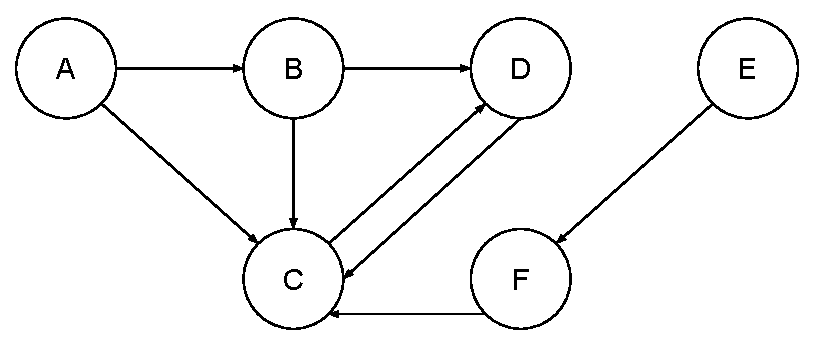
\includegraphics[width=0.8\textwidth]{Pics/Net}
\end{center}

Þetta er mögulegt að gera með hlutbundinni forritun, en einfaldast er að nota dictionary og lista.

\subsection{Breiðleit}

Skrifið breiðleitarreiknirit (e. \emph{breadth-first-search}) sem virkar á netið.

\subsection{Djúpleit}

Skrifið djúpleitarreiknirit (e. \emph{depth-first-search}) sem virkar á netið.


\end{document}